\documentclass[12pt,addpoints]{exam}
\usepackage{enumitem}
\usepackage{amsfonts,amssymb,amsmath, amsthm}
\usepackage{graphicx}
\usepackage{systeme}
\usepackage{pgf,tikz,pgfplots}
\pgfplotsset{compat=1.15}
\usepackage{hyperref}
\usepgfplotslibrary{fillbetween}
\usepackage{mathrsfs}
\usetikzlibrary{arrows}
\usetikzlibrary{calc}
\usepackage{geometry}
\geometry{
	a4paper,
	total={170mm,257mm},
	left=20mm,
	top=12mm,
}
\pagestyle{headandfoot}
%\firstpageheadrule
\runningheader{Homework 2}{}{Page \thepage\ of \numpages}
\runningheadrule
\firstpagefooter{}{}{}
\runningfooter{By Aaron G.K.}{}{Page \thepage\ of \numpages}
\begin{document}
	\title{St John Baptist De La Salle Catholic School, Addis Ababa\\
		\large Grade 11 Physics Homework 2\\
		$2^\text{nd}$ Quarter}
	\maketitle
	\begin{center}
		\fbox{\fbox{\parbox{6in}{\centering
					Notes, and use of other aids is allowed.  Read all directions carefully and write your answers in the space provided.  To receive full credit, you must show all of your work. \textbf{Cheating or indications of cheating and similar answers will be punished accordingly}. 
		}}}
		\subsubsection*{Information}
		\begin{itemize}
			\item The homework is due on \textbf{Thursday}, \textbf{December 4th}.
			\item You should Work on it \textbf{in the newly organized groups} and consult me if you have any questions. As I have reiterated multiple times, cheating between groups will have a serious consequence.
			\item For purposes of neatness and simplicity of grading, you should do the homework on an \textbf{A-4 paper}. However, use your exercise book as a scrapbook.
			\item All answers should be written using a pen. Do not use a pencil. If you make an error, strike a line through it and correct it on the next line.
			\item If you are attempting the \textbf{Advanced Problems}, your submission should be \textbf{via email}. The \textbf{Advanced Problems }have the same deadline as the rest of the problems. 
		\end{itemize}
	\end{center}
	\newpage
	\begin{questions}
			\subsection*{Problems}
			\question[15] Answer the following questions based on the position versus time graph given below of an object moving.
			\begin{center}
				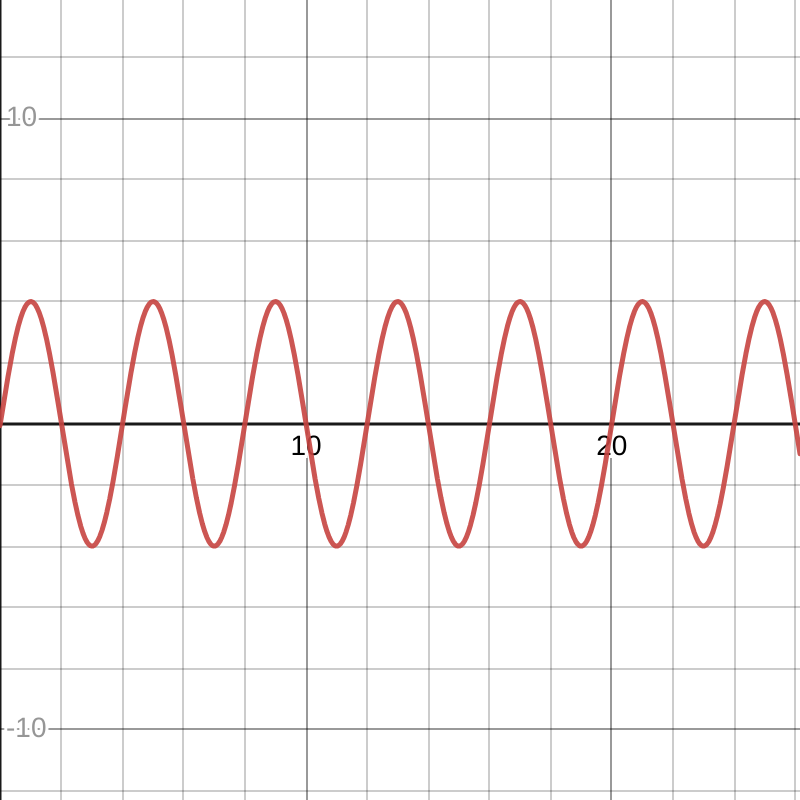
\includegraphics[scale=0.35]{q1.png}
			\end{center}		
		\begin{enumerate}[label=(\Alph*)]
			\item Describe the position as a function of time. 
			\item Find expressions for $v(t)$ and $a(t)$.
			\item Plot the graphs of $v(t)$ and $a(t)$.
			\item What is the jerk 
		\end{enumerate}
		\question[15] The acceleration of a particle moving along the  $x$-axis is given by the equation:
		$$a \left( t \right) = \left(0.500\frac{m}{s^3}\right)t + \left(2.70 \frac{m}{s^2}\right) $$
		If the particle is at position $x=+5.12m$ and is moving in the $-x$
		direction at a speed of $12.8m/s$ at time $t=0s$,
		\begin{enumerate}[label*=(\Alph*)]
			\item Find the time at which the particle momentarily comes to rest.
			\item Find the position where the particle (briefly) comes to rest.
		\end{enumerate}
		\question[10] A ball is thrown vertically upward at the same instant that a second ball is dropped from rest directly above it. The two balls are  $15.0m$ apart when they start their motion. Find the maximum speed at which the first ball can be thrown such that it doesn't collide with the second ball before it returns to its starting height. 
		\question[15] The starting conditions of two cars at $t=0$ are shown in the figure below. The green car, G, starts out 2 $m$ ahead of the pink car, P. At $t=0$ the pink car is moving to the right at 2 $m/s$, while the green car is moving to the right at 5 $m/s$. The pink car is accelerating to the right with magnitude of 6 $m/s^2$, while the green car is accelerating to the left with with magnitude of 4 $m/s^2$. Assume acceleration is constant for both cars. Define the origin at the location of the pink car at  $t=0$.
		\begin{center}
			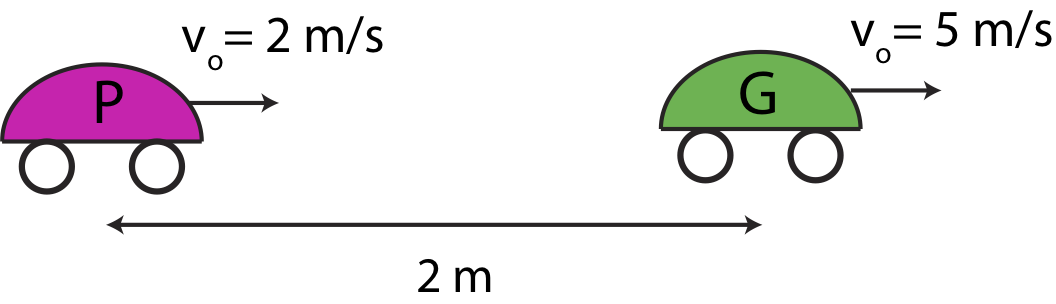
\includegraphics[scale=0.5]{q4.png}
		\end{center}
		\begin{enumerate}[label*=(\Alph*)]
			\item Calculate the time when the pink car catches up to the green one.
			\item At which positions do the two cars meet?
		\end{enumerate}
		\question[15] A car is driving through a green light at $t = 0$ located at $x=0$ with an initial speed $v_{i,c}=16m/s$. At time  $t_1=1s$, the car starts braking until it comes to rest at time $t_2$. The acceleration of the car as a function of time is given by the piece-wise function
		$$a_{c}(t)=\left\{\begin{array}{l} 
			0 ; \quad 0<t<t_{1}=1 \mathrm{s} \\ 
			b\left(t-t_{1}\right) ; 1 \mathrm{s}<t<t_{2} 
		\end{array}\right. \nonumber$$
		where $b = -(8 m/s^3)$.
		\begin{enumerate}[label*=(\Alph*)]
			\item Assuming the car travels only in the x-direction, find the velocity and the position of the car as a function of time.
			\item A bicycle rider is riding at a constant speed of  $V_{i,b}$
			and at $t = 0$ is 32 m behind the car. The bicyclist reaches the car when the car just comes to rest. What is the speed of the bicycle?
		\end{enumerate}
		\question[15] At the instant a traffic light turns green, a car starts from rest with a given constant acceleration, $3.0m/s^{2}$. Just as the light turns green, a bus, traveling with a given constant velocity,  $18m/s$, passes the car. The car speeds up and passes the bus sometime later. How far down the road has the car traveled, when the car passes the bus?
		\question[15] A car, starting at rest at  $t=0$, accelerates in a straight line for 140 m with an unknown constant acceleration. It reaches a speed of 12 $m/s$ and then continues at this speed for another 20 s.
		\begin{enumerate}[label*=(\Alph*)]
			\item Write down the equations for the position and velocity of the car as a function of time.
			\item How long was the car accelerating?
			\item What was the magnitude of the acceleration?
			\item Plot speed vs. time, acceleration vs. time, and position vs. time for the entire motion.
			\item What was the average velocity for the entire trip?
		\end{enumerate}
		\subsection*{Advanced Problems}
		\question[15] Write a simple python program using the normal \href{https://python.org}{python} or \href{https://vpython.org/}{vpython} that models a freely falling object with a specified input initial height \& velocity from a user.
		\begin{enumerate}[label*=(\alph*)]
			\item (5 points) Your program should properly take input.
			\item (5 points) Your program should plot the $v(t)$ \& $x(t)$ graphs.
			\item (2 points) You can make your program prepare an animation/GIF of the trajectory for additional extra credit. 
			\item (3 points) You can upload your program online to Github for extra credit.
		\end{enumerate}
	\end{questions}
\end{document}